\documentclass[10pt]{article}
\usepackage{epsf}
\usepackage{amsmath}
\usepackage{amssymb}
\usepackage{palatino}
\usepackage[pdftex]{graphics}
\usepackage{fancyhdr}
\usepackage{epsfig}
\usepackage{multirow}
\usepackage{multicol}
\usepackage{cancel}
\usepackage{hyperref}
\usepackage{longtable}
\usepackage{ulem}
\usepackage[yyyymmdd]{datetime}
\renewcommand{\dateseparator}{-}
\usepackage{listings}

\parindent 0in
\parskip 1ex
\oddsidemargin  0in
\evensidemargin 0in
\textheight 8.5in
\textwidth 6.5in
\topmargin -0.25in

\pagestyle{fancy}
\lhead{\textbf{\leftheader}}
\rhead{\textbf{\rightheader}}
\lfoot{Compiled: \today\ \currenttime}
\cfoot{}
\rfoot{\thepage}

\newcommand{\leftheader}{BME290L: MedTech Prototyping Skills}
\newcommand{\rightheader}{Palmeri (Spring 2023)}

\begin{document}

\title{Lab 05: Prepare Schematic for PCB Layout} 
\author{MedTech Prototyping Skills (BME290L)}
\maketitle

\section{Update Board to \texttt{v2.1.1}}

\begin{itemize}
    \item Upgrade circuit schematic to \texttt{v2.1.1} (\url{https://mlp6.pages.oit.duke.edu/MedTech-Prototyping-Skills/Prototyping-S23-one-shot-blinking-light-v2.1.0.pdf})\footnote{\texttt{v2.1.1} and \texttt{v2.1.0} have the same rendered schematic.}
    \item Note the \texttt{CHANGELOG} on the schematic.
\end{itemize}

\centerline{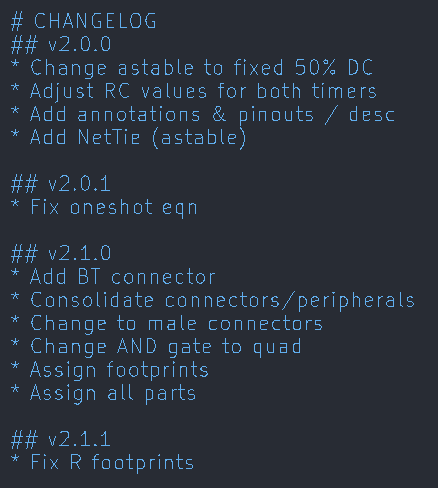
\includegraphics[width=0.4\textwidth]{changelog.png}}

\section{Exclude Peripheral Parts from PCB}

\centerline{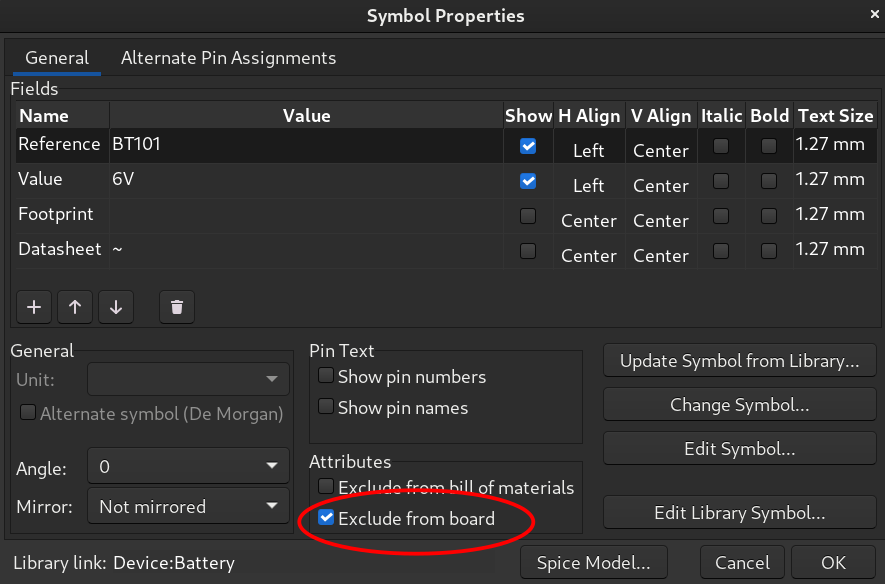
\includegraphics[width=0.5\textwidth]{exclude_from_pcb.png}}

\section{Assign Footprints}

\begin{itemize}
    \item \texttt{Tools -> Assign Footprints\dots}
    \item Can also assign footprints directly to each part (\texttt{Properties})
\end{itemize}

\centerline{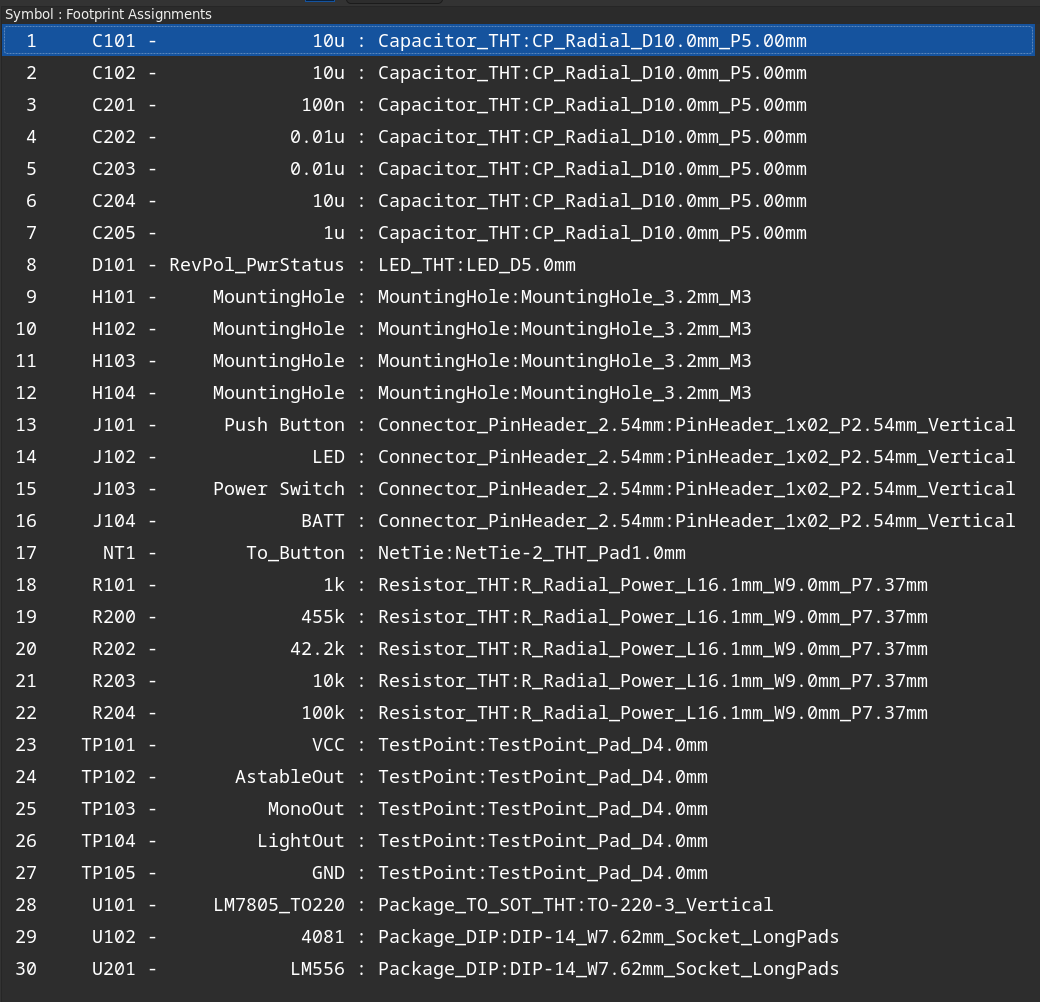
\includegraphics[width=0.75\textwidth]{footprints.png}}

\section{Augment Functionality of Your Circuit}

\begin{itemize}
    \item Modify your circuit to use potentiometers to adjust the LED on-time duration and the blink rate.
    \item Determine the range of your functional modulation with those potentiometers.
    \item Choose your own adventure:
    \begin{enumerate}
        \item Change the output stage of the circuit toggle 2 LEDs out of phase
            with one another, or
        \item Up the ante and come up with a more creative / complex output
            scheme.  Complexity will be rewarded\dots but not at the expense of
            functionality (from a grading perspective).
    \end{enumerate}
\end{itemize}

\section{Generate Bill of Materials}

\begin{itemize}
    \item \texttt{Tools -> Generate BOM\dots} (include footprints)
\end{itemize}

\section{What to Submit}
A single PDF containing:
\begin{itemize}
    \item The sheets of your augmented schematic, versioned at \texttt{v3.x.x}.
    \item Rendered BOM with footprint descriptions.
\end{itemize}

\end{document}
